\documentclass{article}

\usepackage{amsmath}
\usepackage{graphicx}
\usepackage{geometry}
\geometry{margin=1in}

\title{Machine Learning Assignment}
\author{Om Tripathi \ Roll Number: BA2025027}
\date{}

\begin{document}

\maketitle

% ---------------- Q1 ----------------
\section*{Q1: Decision Trees}

\subsection*{(a) Entropy, Gini, Information Gain}

Entropy:
[
H = -(0.6 \log_2 0.6 + 0.4 \log_2 0.4) = 0.971
]

Gini:
[
G = 1 - (0.6^2 + 0.4^2) = 0.48
]

Weighted entropy:
[
H_{split} = 0.891
]

Information gain:
[
IG = 0.08
]

\subsection*{(b) ID3 vs CART}

ID3 selects the split with the highest information gain, while CART selects the split with the lowest Gini impurity. Hence, they may produce different trees.

\subsection*{(c) Overfitting and Bias-Variance Tradeoff}

A fully grown tree overfits the training data due to high variance and performs poorly on unseen data. Increasing depth increases variance. Using constraints like minimum samples split and post-pruning helps reduce overfitting.

\subsection*{(d) Experiment}

\begin{center}
\includegraphics[width=0.7\textwidth]{q1_decision_tree_accuracy.png}
\end{center}

\begin{center}
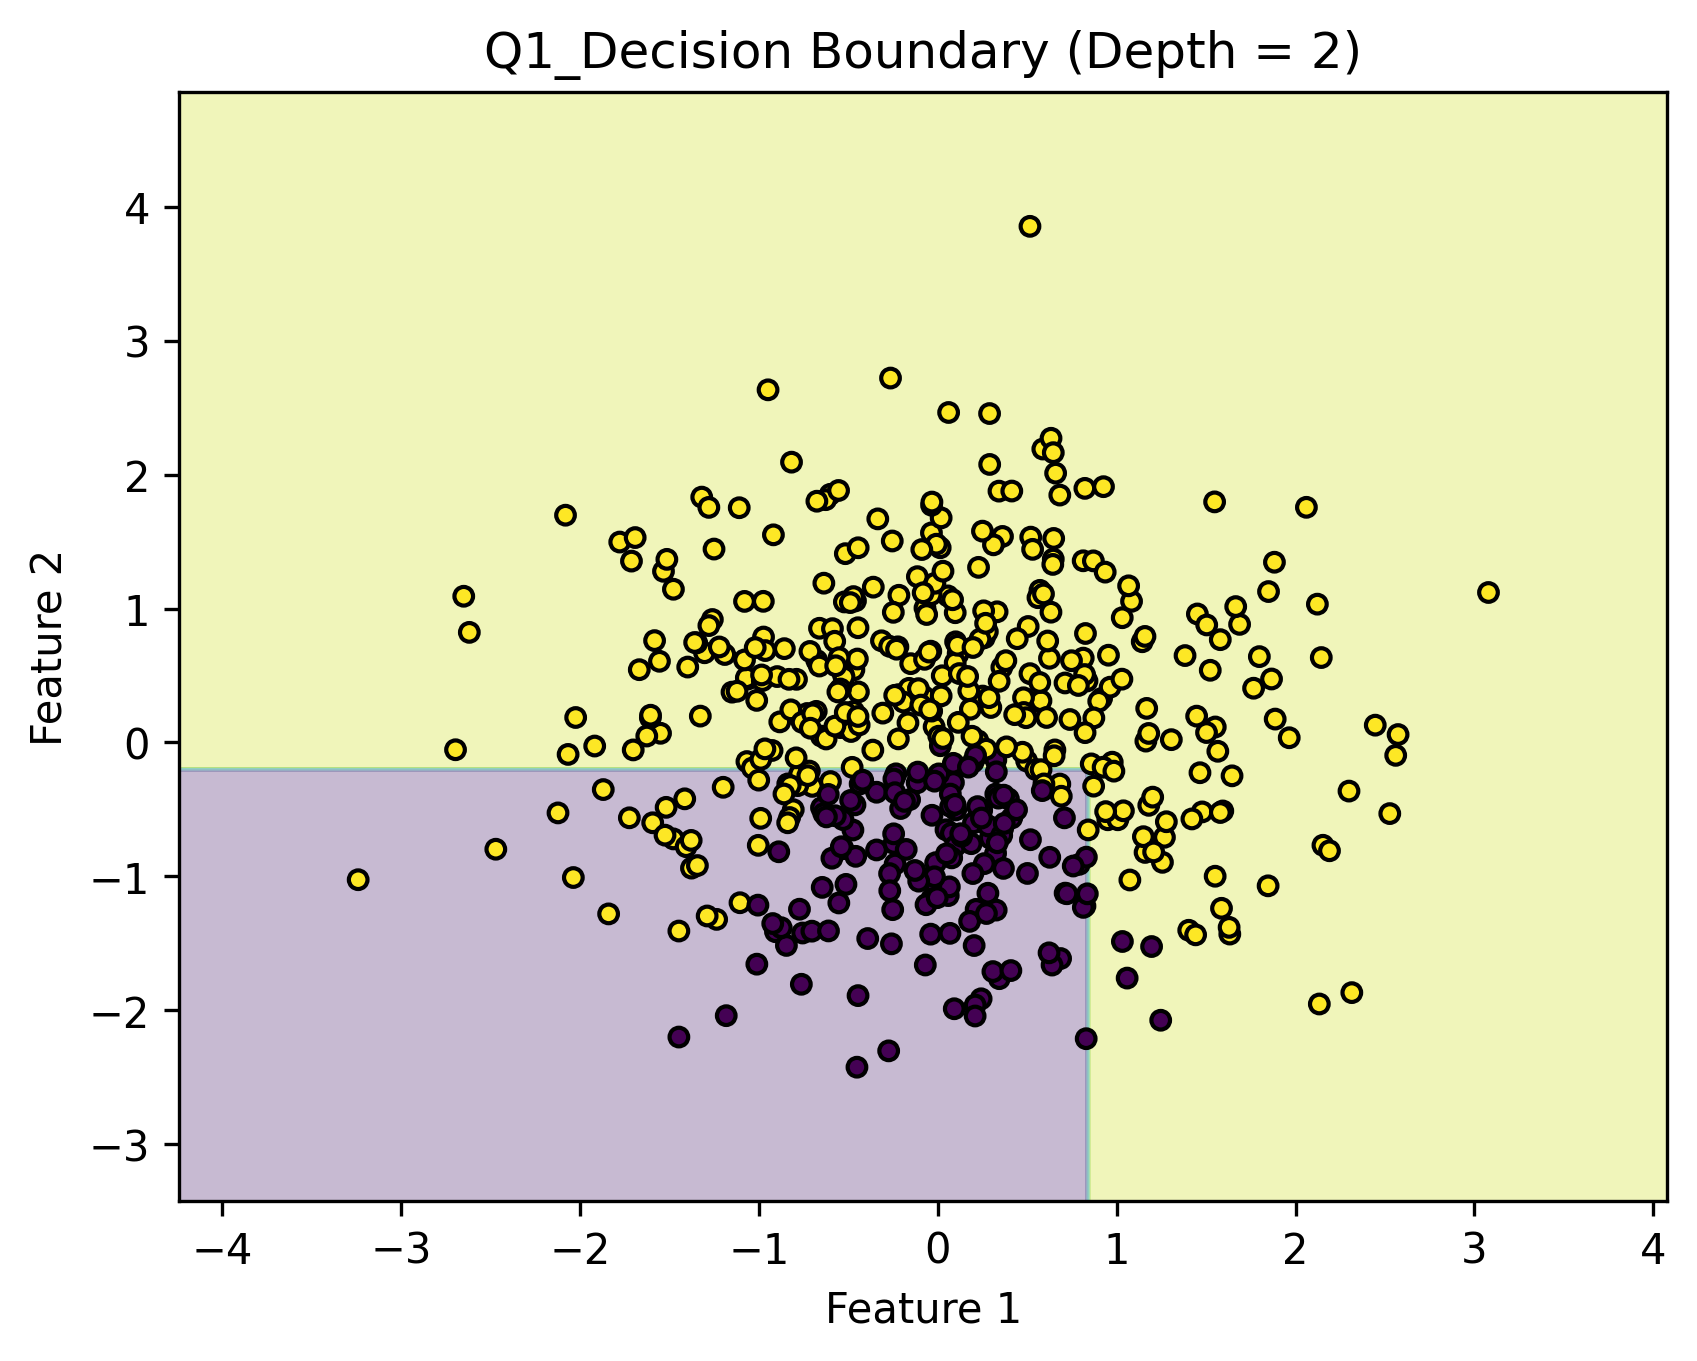
\includegraphics[width=0.45\textwidth]{q1_decision_boundary_depth_2.png}
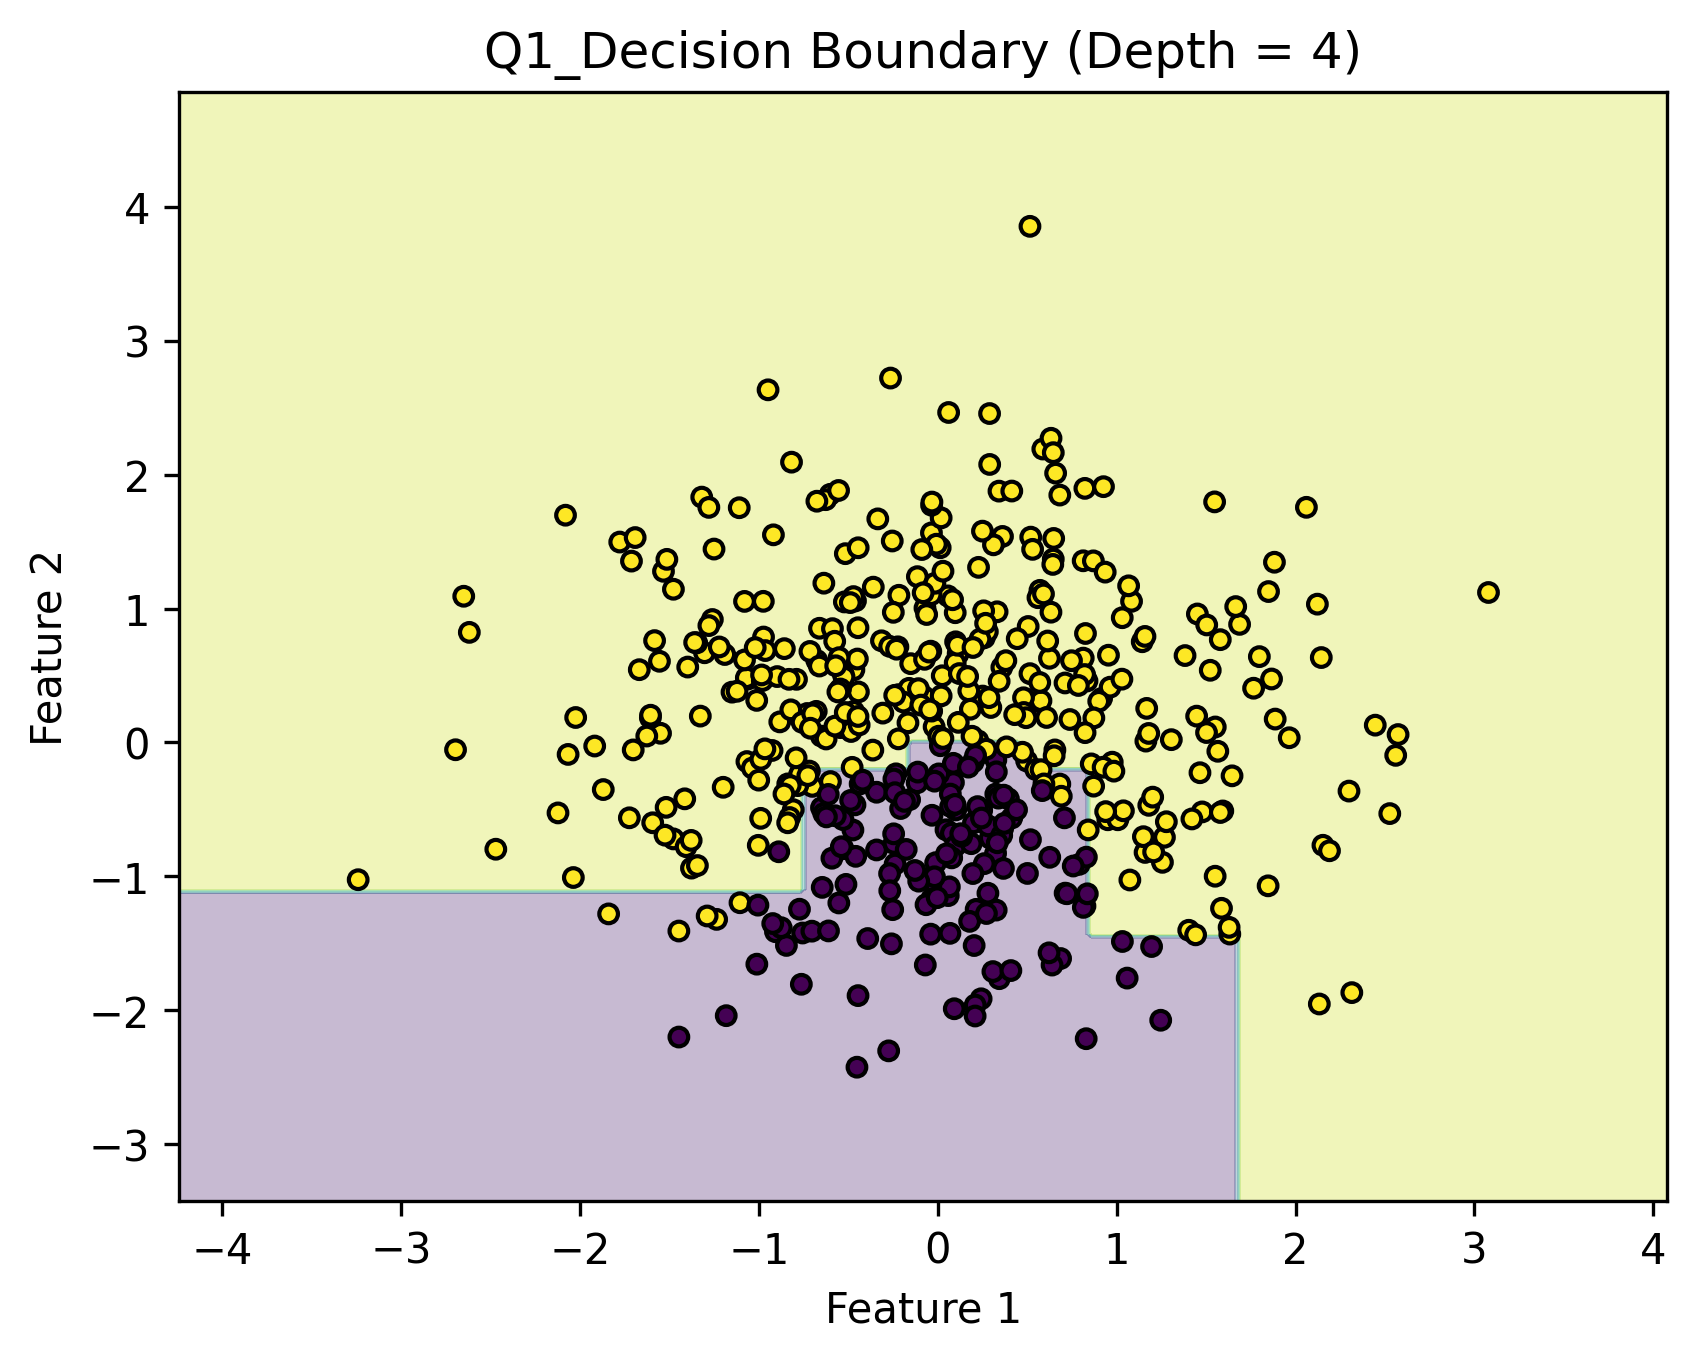
\includegraphics[width=0.45\textwidth]{q1_decision_boundary_depth_4.png}

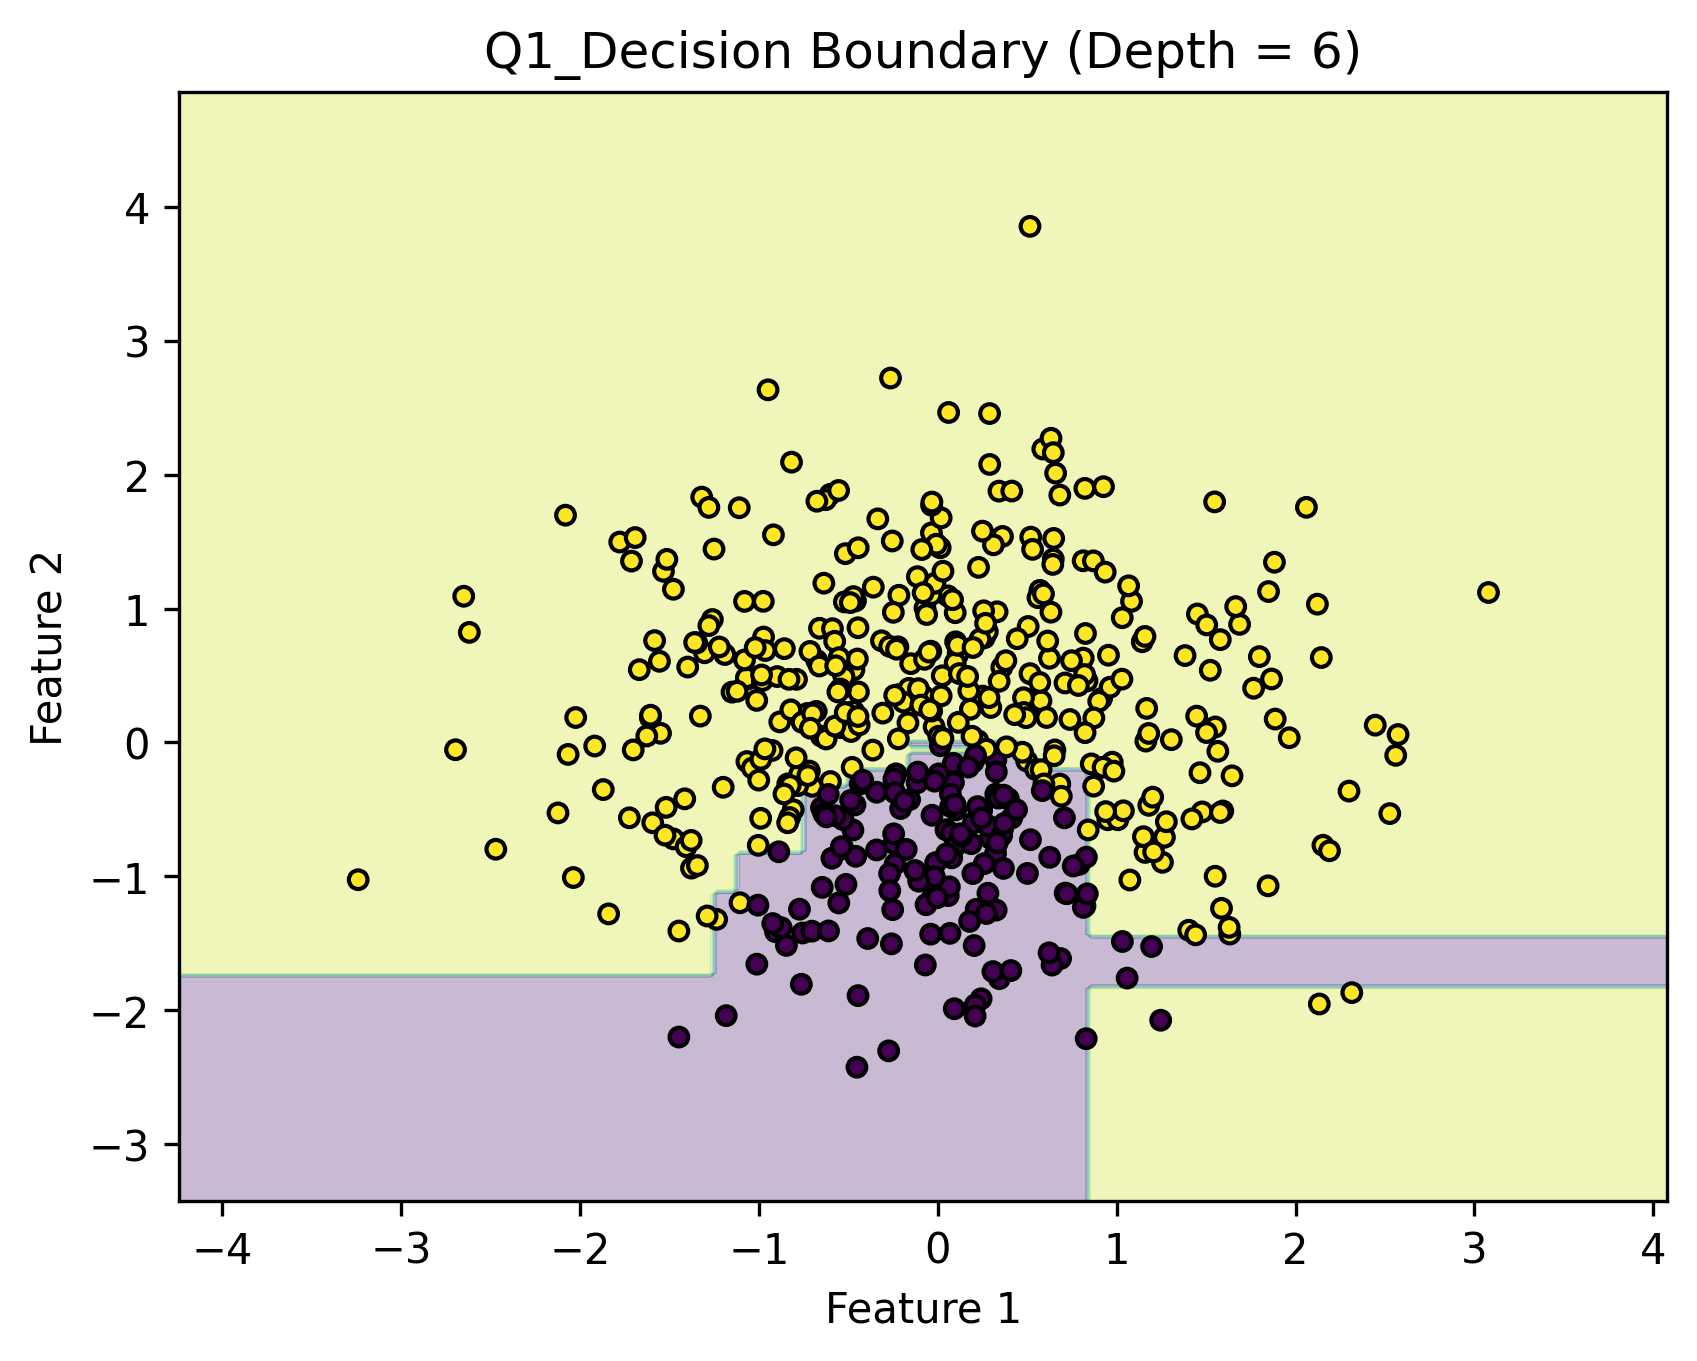
\includegraphics[width=0.45\textwidth]{q1_decision_boundary_depth_6.png}
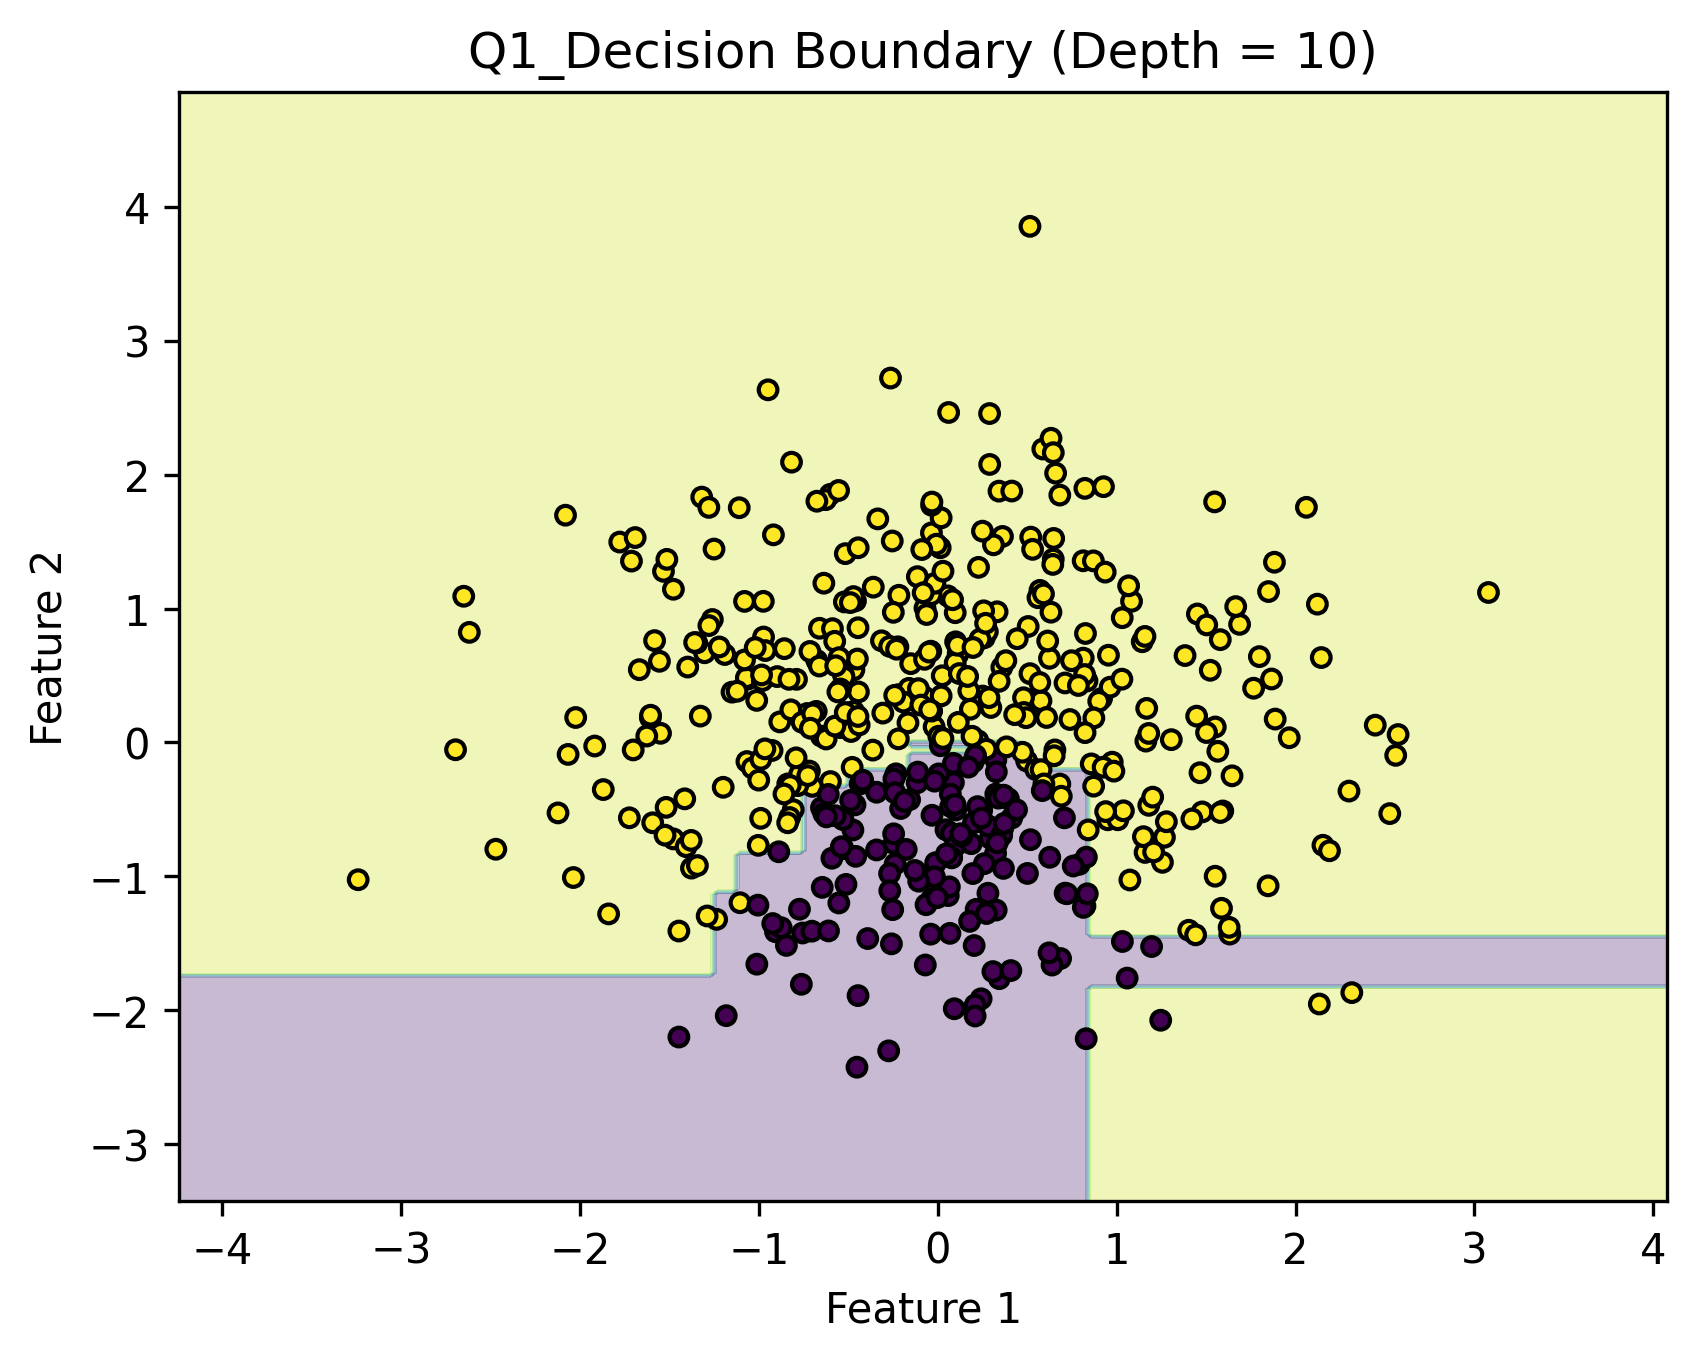
\includegraphics[width=0.45\textwidth]{q1_decision_boundary_depth_10.png}
\end{center}

Training accuracy increases with depth, while testing accuracy initially improves and then decreases, indicating overfitting. Decision boundaries become more complex at higher depths.

% ---------------- Q2 ----------------
\section*{Q2: Logistic Regression}

\subsection*{(a) Log-Likelihood and Gradients}

[
P(Y=1|x) = \frac{1}{1 + e^{-(wx+b)}}
]

[
L = \sum [y \log(\hat{y}) + (1-y)\log(1-\hat{y})]
]

[
\frac{\partial L}{\partial w} = \sum (y - \hat{y})x
\quad
\frac{\partial L}{\partial b} = \sum (y - \hat{y})
]

\subsection*{(b) Numerical Computation}

Predicted probabilities:
[
[0.377, 0.5, 0.622, 0.731]
]

Loss:
[
2.79
]

\subsection*{(c) Linear Decision Boundary}

The decision boundary is linear and defined by:
[
wx + b = 0
]

\subsection*{(d) Implementation}

\begin{center}
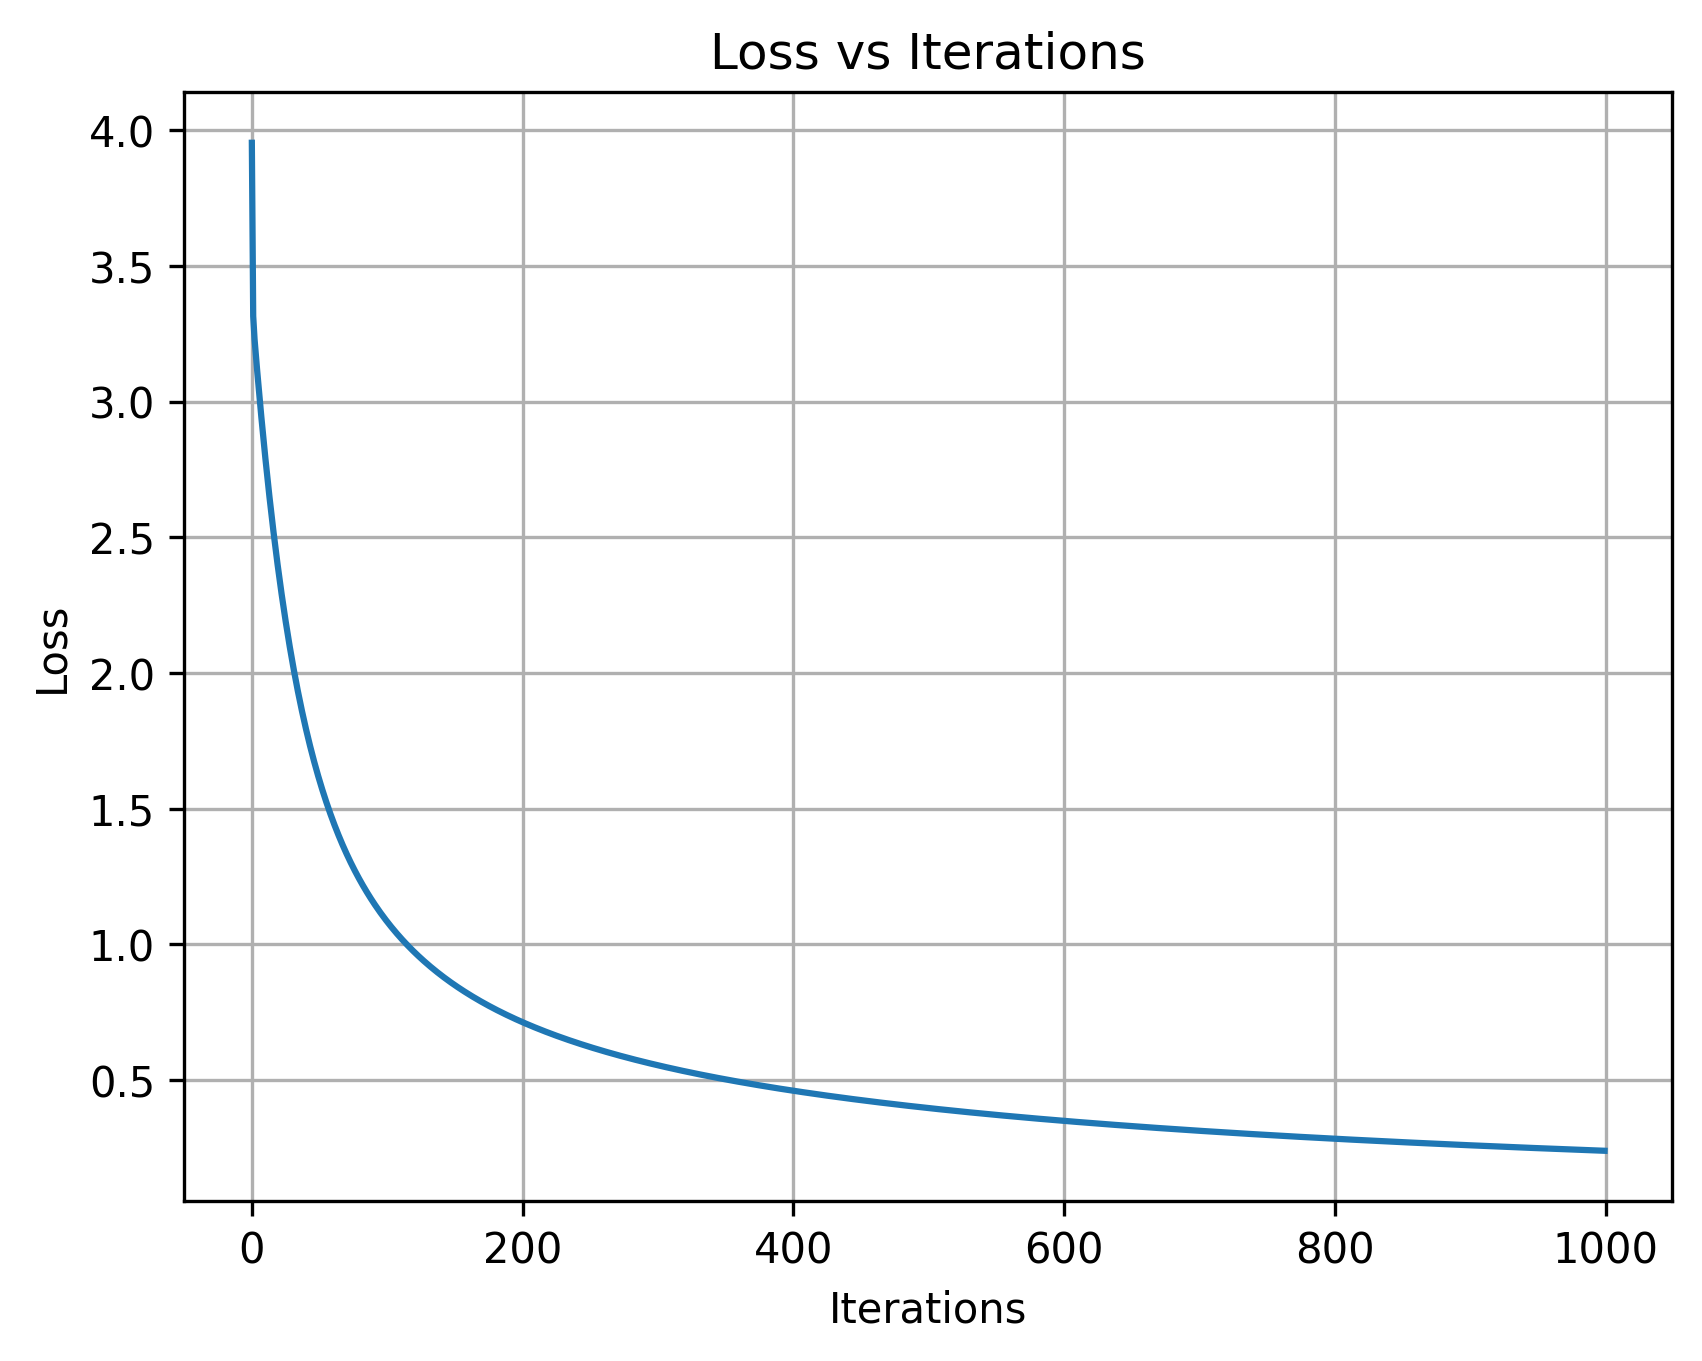
\includegraphics[width=0.7\textwidth]{logistic_loss.png}
\end{center}

The loss decreases over iterations, showing successful convergence of gradient descent.

% ---------------- Q3 ----------------
\section*{Q3: Polynomial Regression}

\subsection*{(a) Normal Equation}

[
\beta = (X^T X)^{-1} X^T y
]

\subsection*{(b) Effect of Degree}

Higher-degree polynomials reduce bias but increase variance, leading to overfitting.

\subsection*{(c) Experiment}

\begin{center}
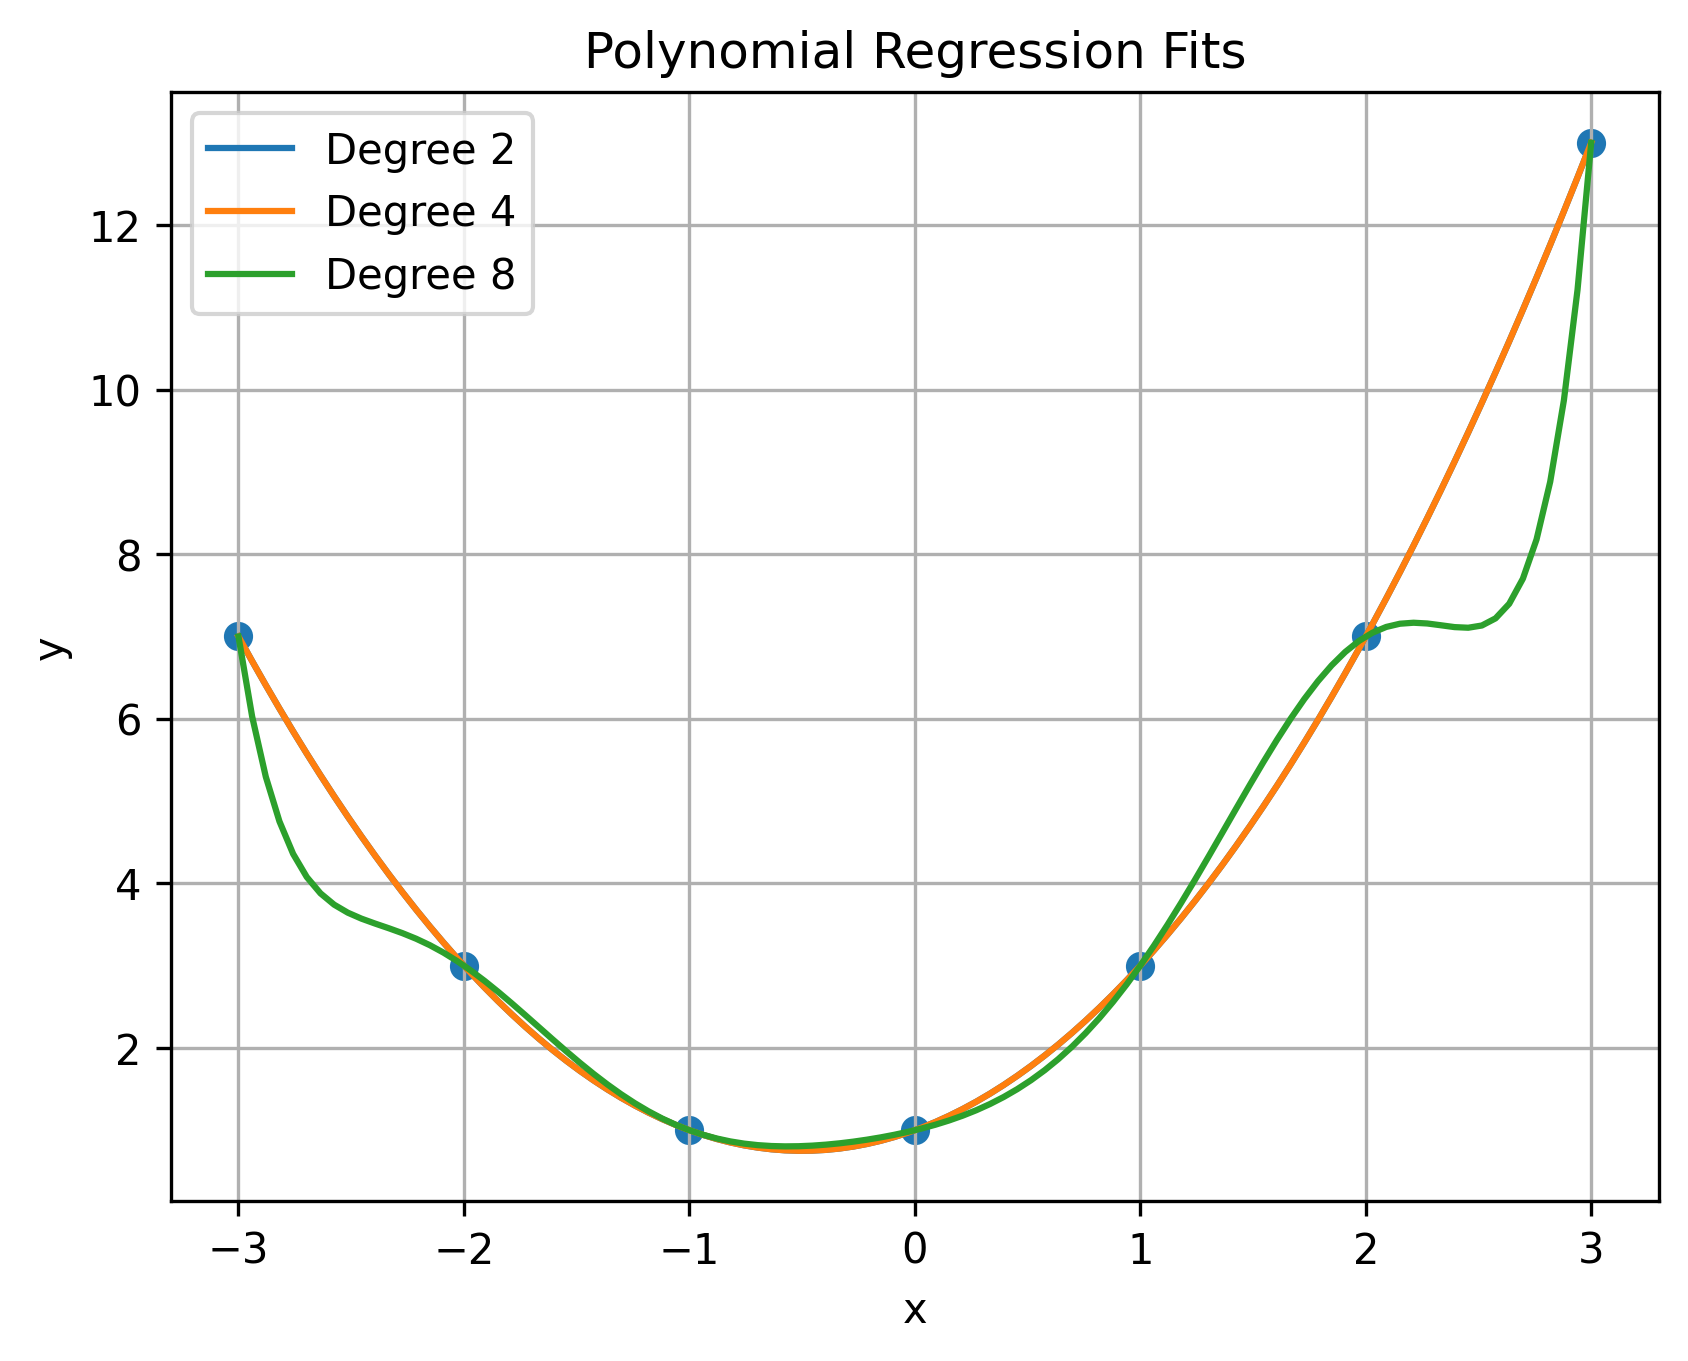
\includegraphics[width=0.7\textwidth]{q3_polynomial_fits.png}
\end{center}

Higher-degree models fit training data better but show oscillatory behavior indicating overfitting.

\subsection*{(d) Ridge Regression}

[
\beta = (X^T X + \lambda I)^{-1} X^T y
]

Increasing $\lambda$ increases bias and reduces variance.

% ---------------- Q4 ----------------
\section*{Q4: K-Means Clustering}

\subsection*{(a) One Iteration}

Updated centroids:
[
(1.25, 1.5), \quad (3.9, 5.1)
]

\subsection*{(b) Objective Function}

[
J = \sum |x - \mu|^2
]

\subsection*{(c) Local Minima}

K-means may converge to different solutions depending on initialization.

\subsection*{(d) Implementation}

\begin{center}
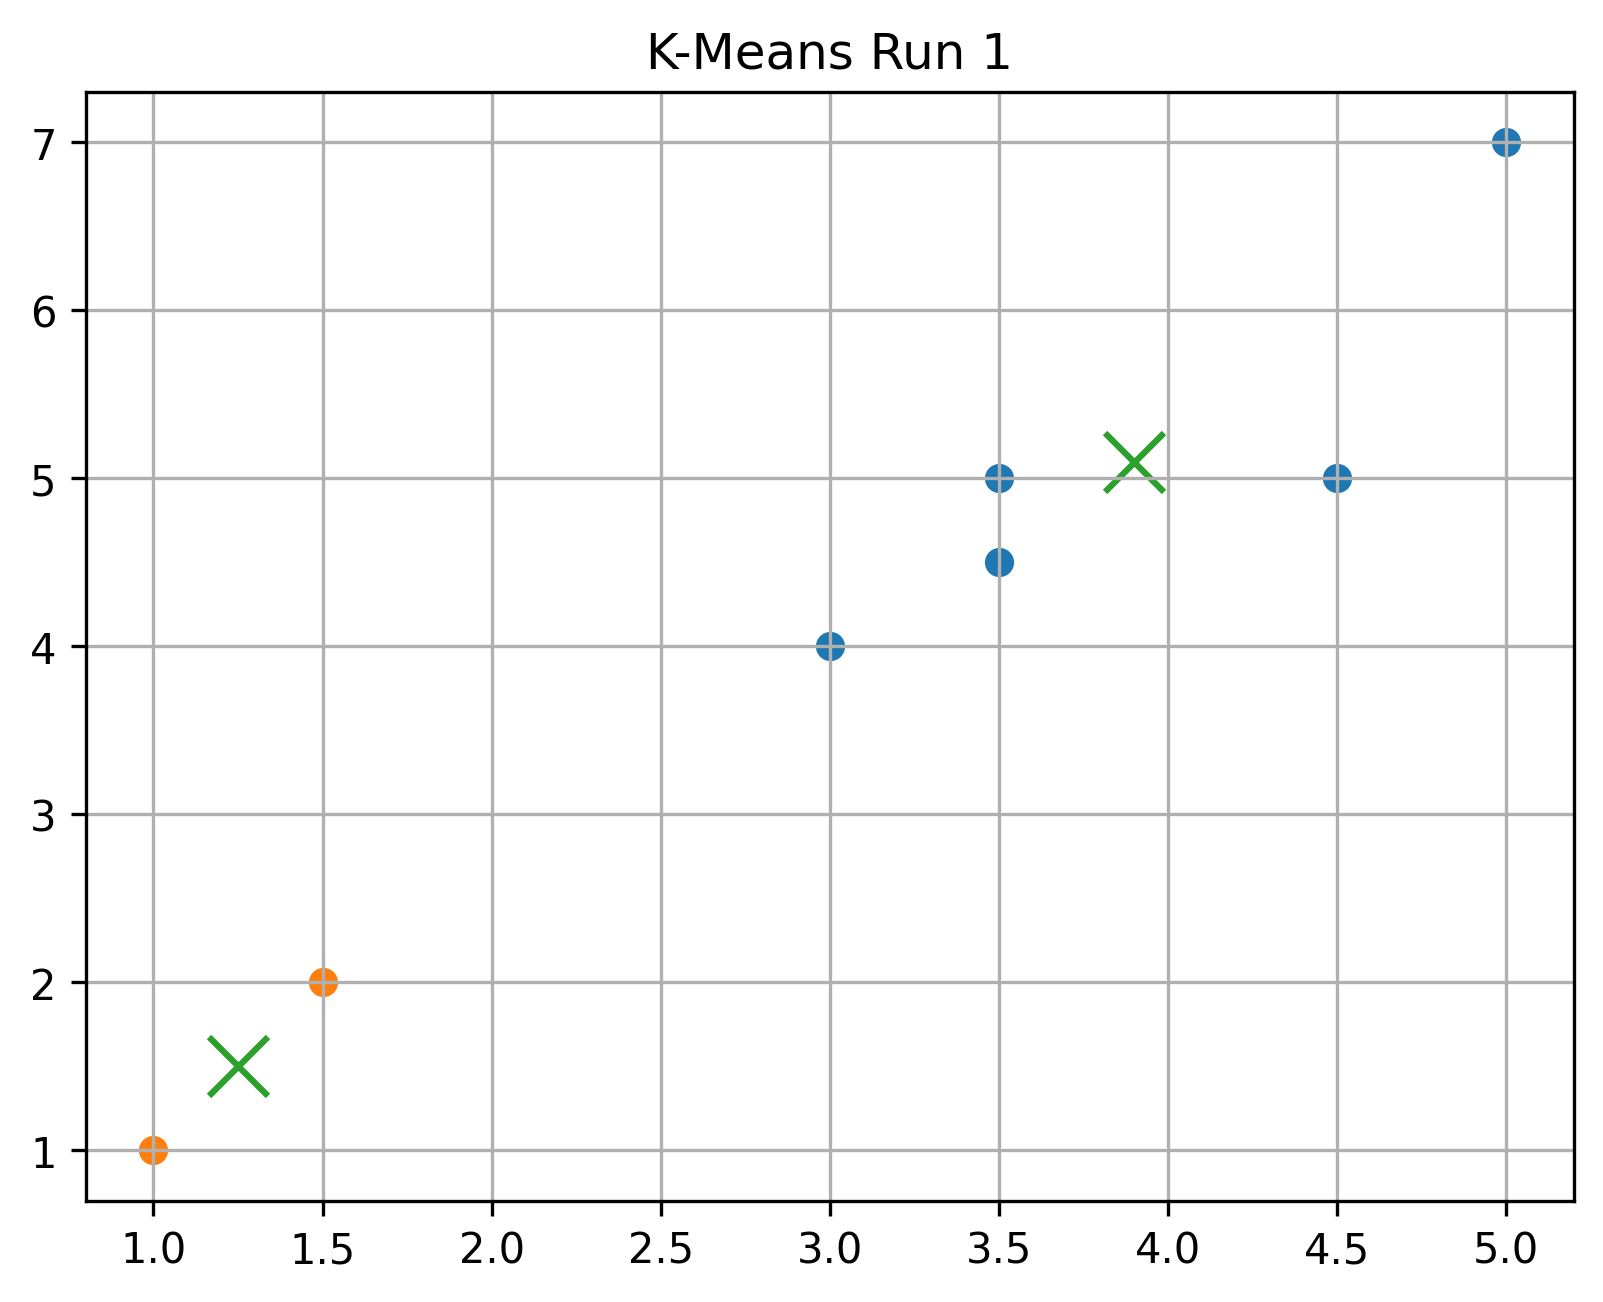
\includegraphics[width=0.45\textwidth]{q4_kmeans_run_1.png}
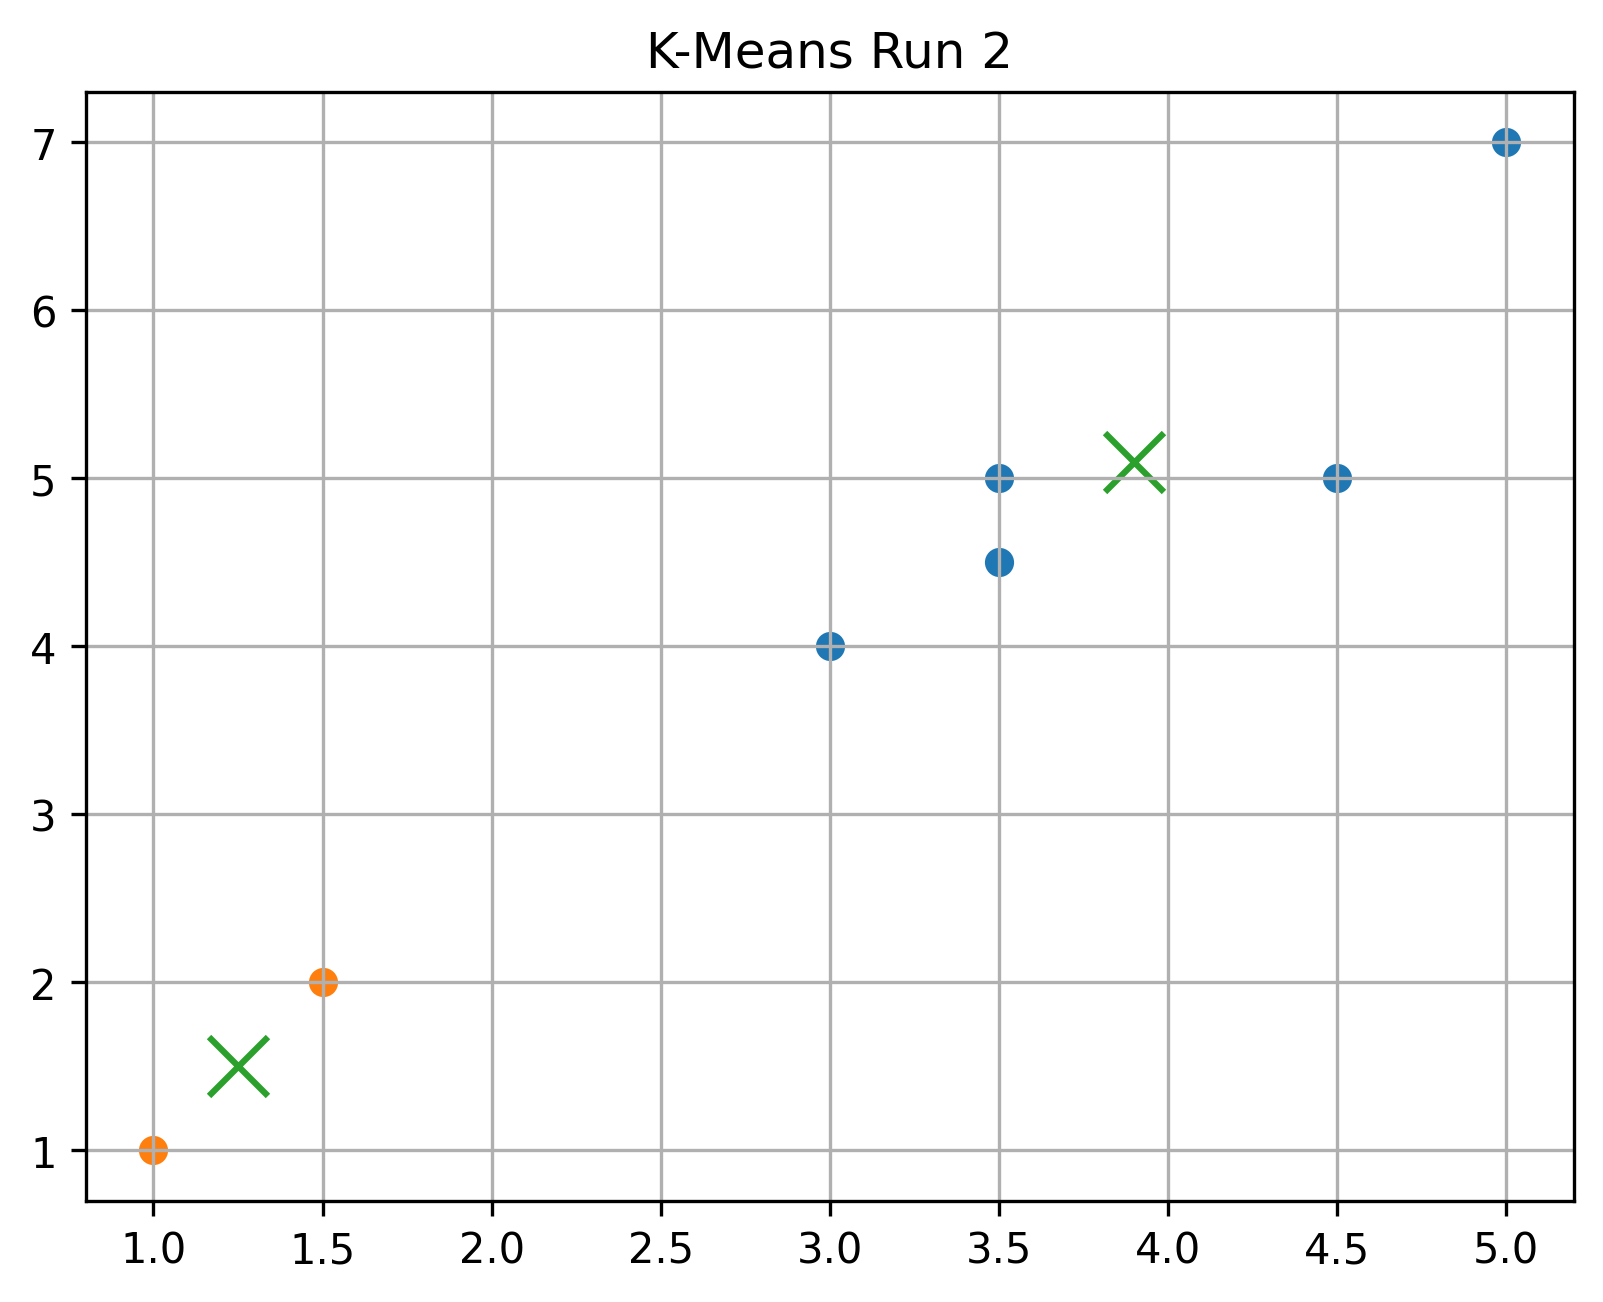
\includegraphics[width=0.45\textwidth]{q4_kmeans_run_2.png}
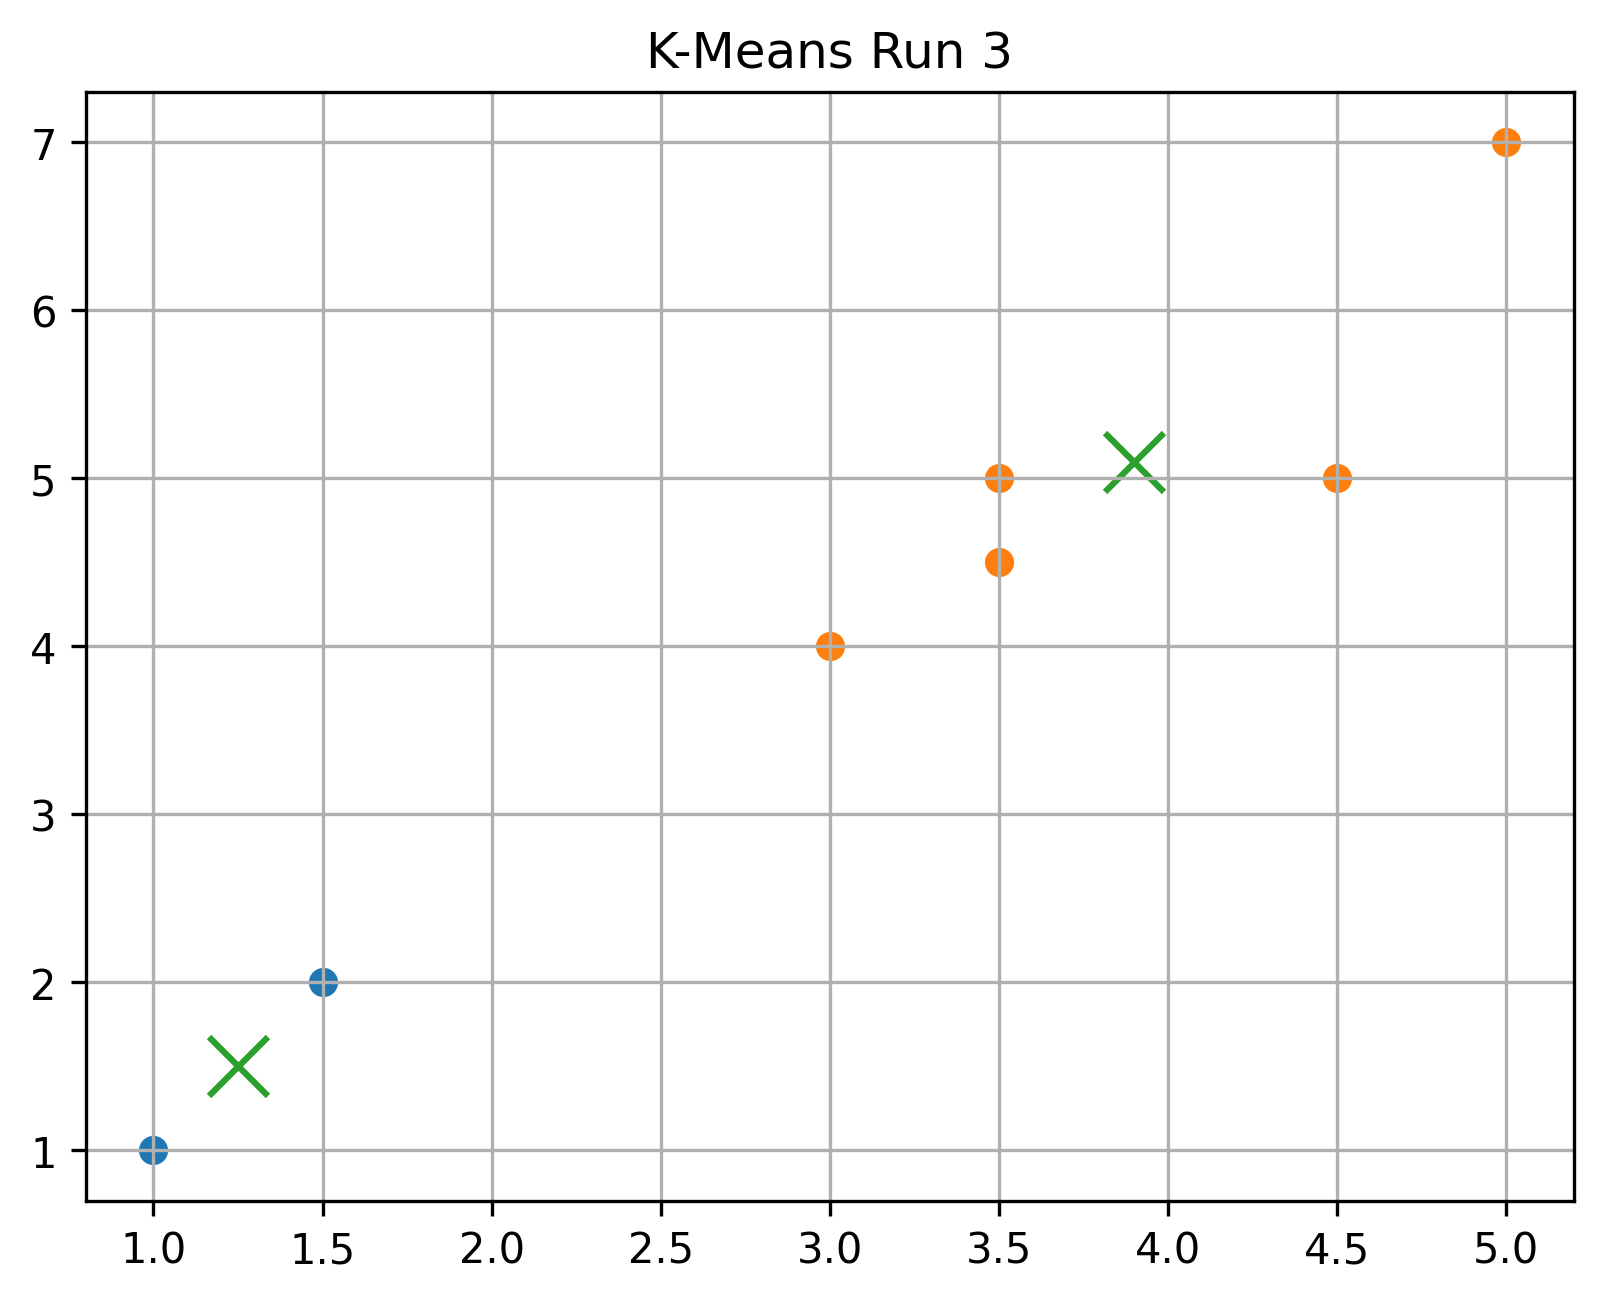
\includegraphics[width=0.45\textwidth]{q4_kmeans_run_3.png}
\end{center}

Different runs produce different cluster assignments and SSE values.

\end{document}
